\documentclass[conference]{IEEEtran}
\IEEEoverridecommandlockouts
\usepackage{cite}
\usepackage{amsmath,amssymb,amsfonts}
\usepackage{algorithmic}
\usepackage{graphicx}
\usepackage{textcomp}
\usepackage{xcolor}
\usepackage{subcaption}
\def\BibTeX{{\rm B\kern-.05em{\sc i\kern-.025em b}\kern-.08em
    T\kern-.1667em\lower.7ex\hbox{E}\kern-.125emX}}
\begin{document}

\title{Bad Beginnings:\\ Why the Observation Model, Not the Filter, Decides\\ Localization Recovery under Wrong Initialization}

\author{\IEEEauthorblockN{Elias Bitsch}
\IEEEauthorblockA{Probabilistic Robotics Lab\\
University of Applied Sciences Technikum Wien\\
Vienna, Austria}}

\maketitle

\begin{abstract}
Recursive Bayesian filters are the workhorse of mobile-robot localization, but their textbook guarantees assume an approximately correct initial belief. In real deployments this assumption breaks: a robot is switched on at an unknown pose, is given a wrong start by an operator, or is physically displaced. We present a controlled, reproducible comparison of five localization filters, namely a linear Kalman filter, an extended Kalman filter with fiducial landmarks, an extended Kalman filter with a scan likelihood field, a Monte Carlo particle filter, and the Nav2 adaptive Monte Carlo baseline, across seven deliberately adverse initialization scenarios on a TurtleBot~4 in a perceptually symmetric warehouse. The four research filters are implemented from first principles. Landmark identity is obtained honestly from a camera that reads AprilTag fiducials, not from a ground-truth oracle. Over ten random seeds per scenario we find a sharp and consistent split: filters that observe distinguishable landmark identity recover from large offsets, wrong heading, miscalibrated covariance, and even double kidnapping, whereas scan-based filters, including the de-facto standard, are defeated by perceptual aliasing and diverge by up to seventeen metres. Crucially, this advantage vanishes under nominal conditions, where all filters localize to within fifteen centimetres and corrections merely add noise. The decisive factor for recovery is therefore the identifiability of the observation model, not the sophistication of the estimator. All code, the simulation, and the raw data are openly available for verification.
\end{abstract}

%%%%%%%%%%%%%%%%%%%%%%%%%%%%%%%%%%%%%%%%%%%%%%%%%%%%%%%%%%%%%%%%%%
\section{Introduction}

Localization, estimating the pose of a robot inside a known map, is a prerequisite for almost every autonomous task, and recursive Bayesian filtering is its dominant formalism~\cite{Thrun2005}. The Kalman filter~\cite{Kalman1960} and its extended variant, together with Monte Carlo localization~\cite{Dellaert1999}, all share the same recursive structure: a motion model propagates the belief and a measurement model corrects it. Their elegance comes with a quiet assumption, namely that the initial belief already covers the true pose. When it does not, the very mechanism that makes these filters efficient, the contraction of the belief around a single hypothesis, works against recovery.

This failure mode is not academic. A warehouse robot is powered up at an arbitrary aisle; an operator clicks a wrong ``2D pose estimate''; a forklift nudges a robot two metres sideways. The extreme case, where the robot is teleported without notice, is the classical \emph{kidnapped-robot problem}~\cite{Thrun2005}. Recovery is further complicated by the environments where such robots work: warehouses are deliberately regular, with repeating racking and pillars, so that many places look alike to a range sensor. This \emph{perceptual aliasing}~\cite{Cummins2008,Lowry2016} means that a geometrically faithful scan can still be consistent with several mutually distant poses.

The robotics community offers two broad answers to ``where am I?'': match raw range scans against the map, as Nav2's adaptive Monte Carlo localization (AMCL) does~\cite{Macenski2023Nav2}, or observe distinguishable artificial landmarks such as visual fiducials~\cite{Olson2011}. These two sensing modalities are usually studied in isolation and under benign initialization. It is not obvious which one matters when the start is wrong: does a more elaborate filter help, or does the choice of \emph{what is measured} dominate?

\textbf{Contribution.} We provide a controlled, multi-seed, reproducible answer. We implement four filters from first principles and stress-test them, alongside the AMCL baseline, across seven adverse-initialization scenarios in a symmetric warehouse, using honest camera-based AprilTag identity for the landmark filters. We show (i) that landmark-identity filters recover from every adverse start while scan-based filters diverge under perceptual aliasing; (ii) that this robustness is specific to bad initialization and disappears under nominal conditions; and (iii) that the deciding factor is the identifiability of the observation model rather than the estimator's complexity. The remainder of the paper reviews related work (Sec.~II), describes the system, filters, and protocol (Sec.~III), presents and discusses results (Sec.~IV), and concludes (Sec.~V).

%%%%%%%%%%%%%%%%%%%%%%%%%%%%%%%%%%%%%%%%%%%%%%%%%%%%%%%%%%%%%%%%%%
\section{State of the Art}

\textbf{Gaussian filters.} The Kalman filter is the optimal linear-Gaussian estimator~\cite{Kalman1960}; the extended Kalman filter (EKF) linearizes a nonlinear motion and measurement model around the current estimate~\cite{Thrun2005}, and the unscented variant avoids explicit Jacobians~\cite{Julier2004}. All maintain a single Gaussian, which is compact and cheap but unimodal: it cannot represent ``I am in one of eight identical aisles.'' Recovery from a gross error is therefore only possible if the measurement uniquely pins the pose.

\textbf{Sample-based filters.} Monte Carlo localization (MCL)~\cite{Dellaert1999} represents the belief by weighted particles and so handles multi-modal, global uncertainty. AMCL adapts the sample count~\cite{Fox2003} and underpins the Nav2 navigation stack~\cite{Macenski2023Nav2}. Plain MCL cannot recover from kidnapping because resampling only redistributes existing hypotheses; augmented MCL injects random particles when the measurement likelihood collapses~\cite{Thrun2005}, which is the textbook remedy for the kidnapped-robot problem.

\textbf{Sensing modalities.} Scan-based correction compares a laser scan against an occupancy map via the likelihood field~\cite{Thrun2005}. It needs no environment modification but is vulnerable to aliasing in repetitive scenes~\cite{Cummins2008,Lowry2016}. Visual fiducials such as AprilTag~\cite{Olson2011,Wang2016} instead provide a uniquely identified, accurately localized landmark, turning the hard data-association problem~\cite{Neira2001} into a solved one at the cost of instrumenting the environment.

\textbf{So what.} Existing comparisons typically assume good initialization, use distinguishable environments, or evaluate a single modality. The interaction that matters for real deployments, namely how the \emph{observation model} governs recovery from a \emph{wrong start} in an \emph{aliased} environment, is rarely isolated. We close this gap with a like-for-like experiment in which every filter receives the same motion and the same adverse initial belief, and only the measurement modality differs.

%%%%%%%%%%%%%%%%%%%%%%%%%%%%%%%%%%%%%%%%%%%%%%%%%%%%%%%%%%%%%%%%%%
\section{Materials and Methods}

\subsection{Platform and simulation}
All experiments run on a simulated TurtleBot~4 (differential drive) in Gazebo~\cite{Koenig2004} under ROS\,2~\cite{Macenski2022ROS2}. The robot exposes wheel odometry, an IMU, a 360$^\circ$ 2D lidar, and an OAK-D RGB camera. The world is a $30\times20$\,m warehouse containing eight steel I-beam pillars arranged in a regular $2\times4$ grid at $7.5$\,m spacing; this regularity is the source of the perceptual aliasing we study. Nav2's AMCL~\cite{Macenski2023Nav2} serves as the baseline. The four research filters (KF, EKF, EKF-LF, PF) are implemented in C++ from first principles; only the sensor frontend and plotting are scripted. Ground truth is taken directly from the simulator and is used \emph{only} to score error, never as a filter input. Fig.~\ref{fig:dataflow} shows the ROS\,2 data flow: which topics enter each filter and what it publishes.

\begin{figure*}[!t]
    \centering
    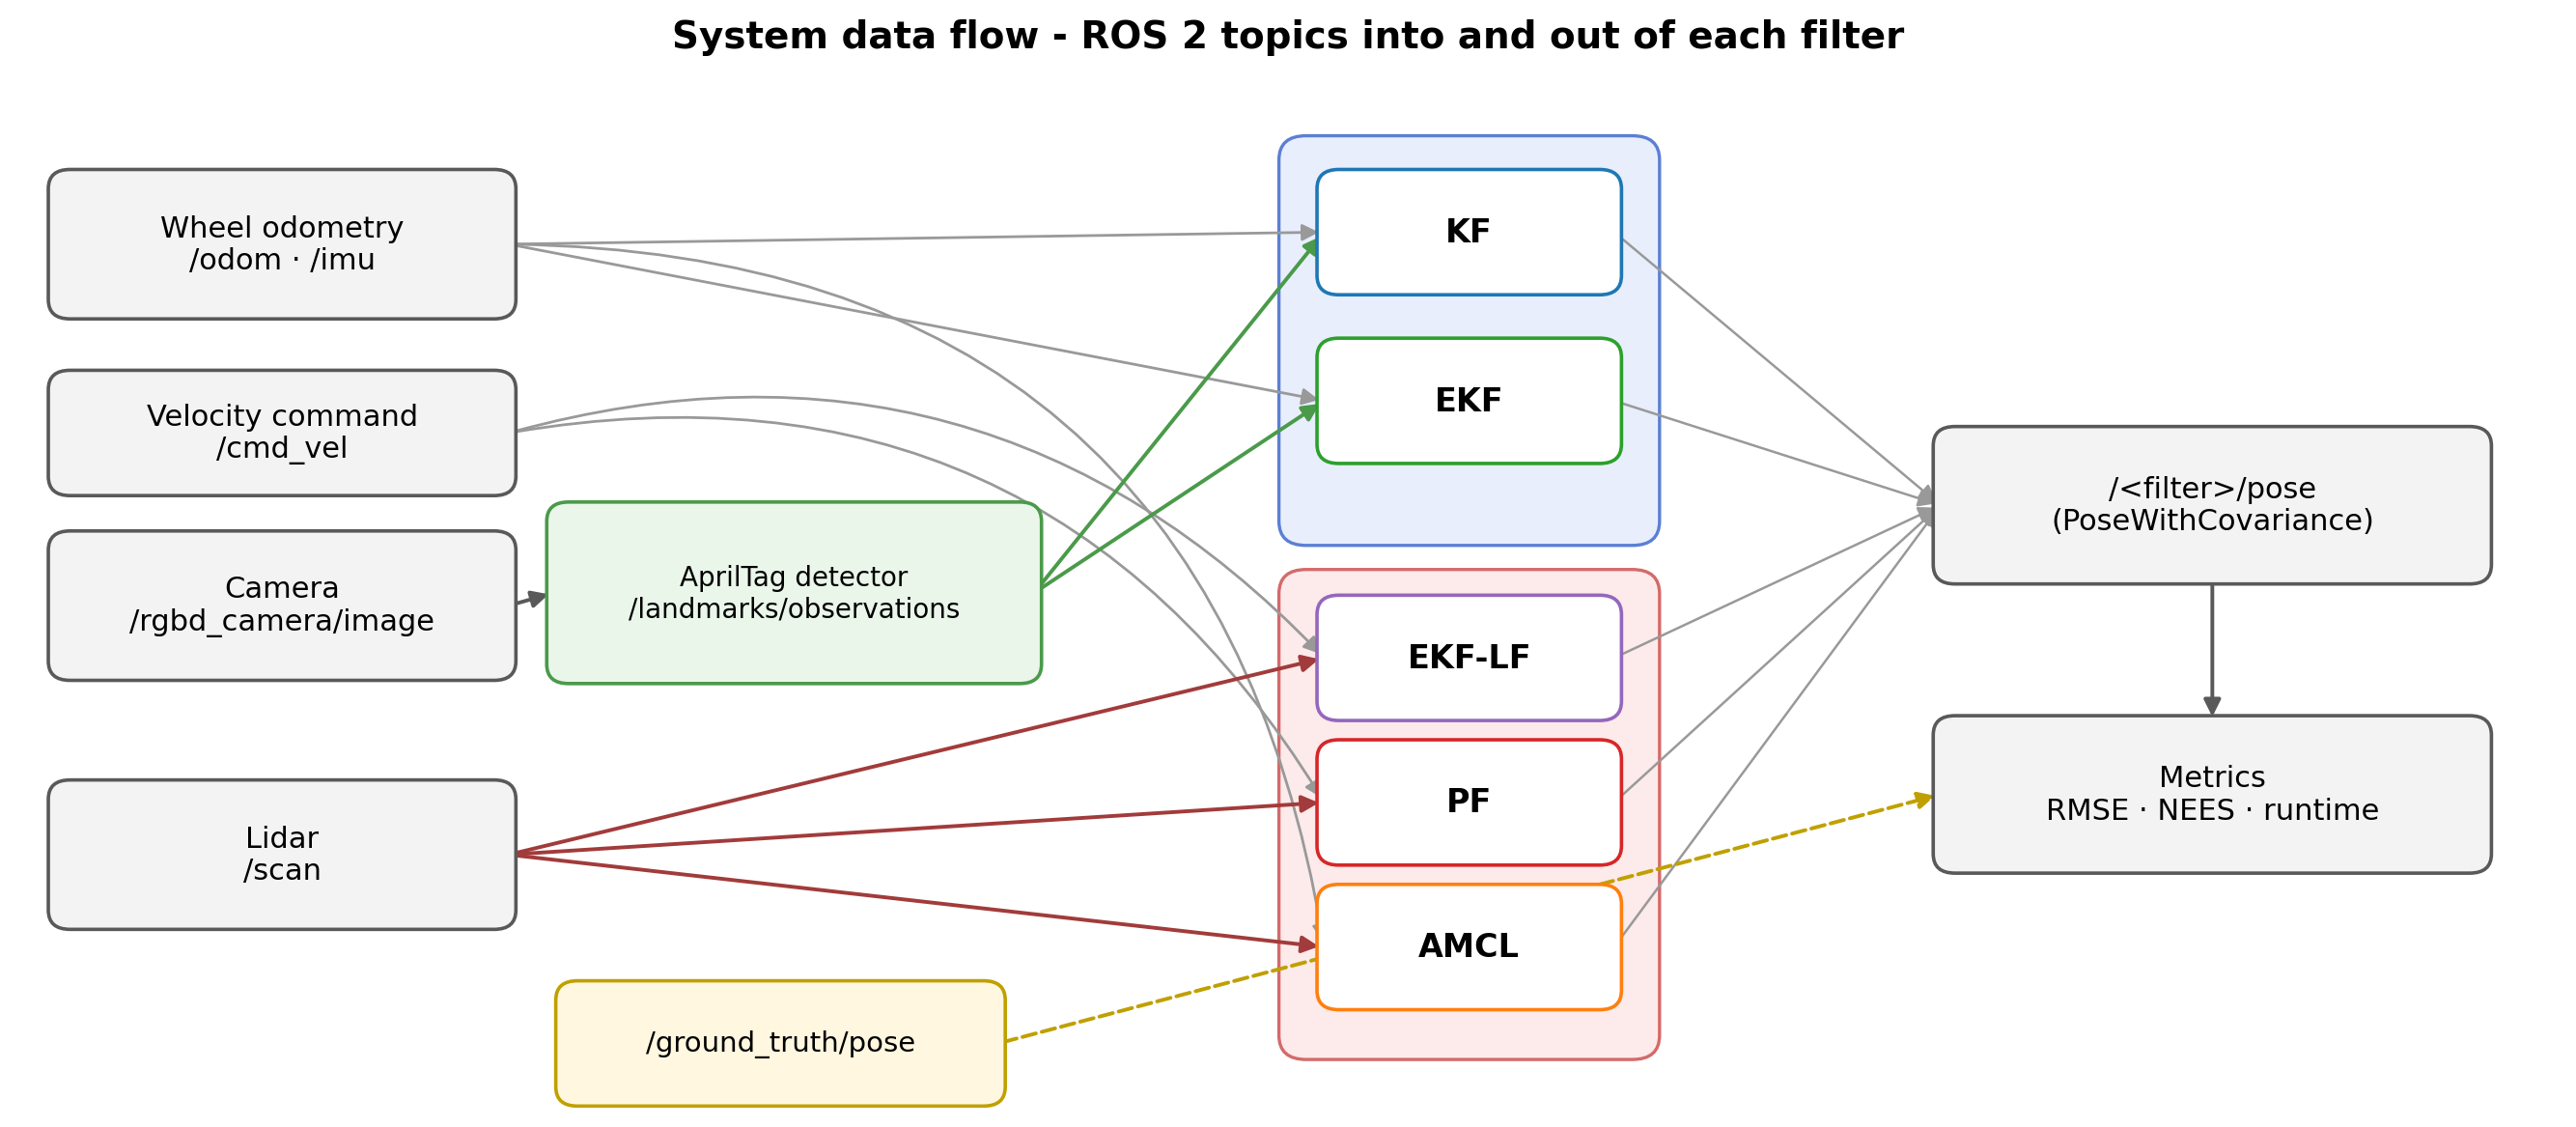
\includegraphics[width=0.96\textwidth]{images/dataflow.png}
    \caption{System data flow. Wheel odometry (\texttt{/odom}) and the IMU drive the motion model of KF, EKF and EKF-LF (and AMCL via TF); the PF instead uses the \texttt{/cmd\_vel} velocity command. The camera image is turned by the AprilTag detector into \texttt{/landmarks/observations}, consumed by the landmark filters (KF, EKF), while \texttt{/scan} drives the scan filters (EKF-LF, PF, AMCL). Each filter publishes \texttt{/<filter>/pose}; ground truth feeds the metrics only, never a filter.}
    \label{fig:dataflow}
\end{figure*}

\subsection{Motion and measurement models}
All filters consume the same control input. The EKF uses the odometry motion model~\cite{Thrun2005} on the unicycle state $\mathbf{x}=(x,y,\theta)^\top$, propagating
\begin{equation}
\mathbf{x}_t = \mathbf{x}_{t-1} +
\begin{bmatrix} \Delta s\cos(\theta_{t-1}+\tfrac{\Delta\theta}{2})\\ \Delta s\sin(\theta_{t-1}+\tfrac{\Delta\theta}{2})\\ \Delta\theta \end{bmatrix},
\end{equation}
with covariance $\mathbf{P}_t=\mathbf{G}_t\mathbf{P}_{t-1}\mathbf{G}_t^\top+\mathbf{R}_t$, where $\mathbf{G}_t$ is the motion Jacobian. The linear KF uses a six-dimensional constant-velocity model as a deliberately simple reference. The \emph{landmark} filters (KF, EKF) correct on a range--bearing observation of a known map landmark $\mathbf{m}_i=(m_{i,x},m_{i,y})$,
\begin{equation}
\mathbf{z}=\begin{bmatrix} r \\ \phi \end{bmatrix}=
\begin{bmatrix} \sqrt{(m_{i,x}-x)^2+(m_{i,y}-y)^2} \\ \mathrm{atan2}(m_{i,y}-y,\,m_{i,x}-x)-\theta \end{bmatrix}+\mathbf{v},
\end{equation}
with the standard EKF gain $\mathbf{K}_t=\mathbf{P}_t\mathbf{H}_t^\top(\mathbf{H}_t\mathbf{P}_t\mathbf{H}_t^\top+\mathbf{Q})^{-1}$. The measurement noise $\mathbf{Q}$ is fixed and identical for both landmark filters; it is not tuned per filter, so the comparison reports raw filter behaviour. The \emph{scan} filters instead correct on the lidar through the likelihood field model~\cite{Thrun2005}: EKF-LF folds the scan-likelihood gradient into an EKF update, while the PF weights each particle by the scan likelihood. The PF uses augmented MCL~\cite{Thrun2005} with random-particle injection so that it can, in principle, recover from kidnapping.

\subsection{Honest landmark identity via AprilTag}
The decisive design choice is that landmark \emph{identity} is measured, not assumed. Each pillar carries a unique AprilTag~\cite{Olson2011} of the \texttt{tag36h11} family. The robot's RGB camera ($1280\times720$) detects tags with the AprilTag-3 detector; the tag corners and known tag size yield the full tag pose by perspective-$n$-point, from which we derive the range, bearing, and, most importantly, the tag identity that selects the map landmark in~(2). No ground-truth pose enters this pipeline. Against simulator ground truth the resulting measurements are accurate to below one centimetre in range and $0.25^\circ$ in bearing. Because the camera looks forward ($\approx 71^\circ$ field of view), the robot typically sees only one tag at a time, a realistic limitation that yields sparser and geometrically weaker updates than an omnidirectional sensor.

\subsection{Scenarios, metrics, and protocol}
We define seven scenarios that share the same scripted trajectory but differ in the initial belief: \texttt{correct\_init} (nominal); \texttt{offset\_1m} and \texttt{offset\_5m} (translated start); \texttt{wrong\_yaw\_pi2} ($90^\circ$ heading error); \texttt{overconfident\_wrong} (wrong start with a tight covariance); \texttt{underconfident} (correct start with an inflated covariance); and \texttt{kidnapped} (two unannounced teleports during the run). For each filter we report the position error RMSE$_{xy}$, the convergence rate (the fraction of seeds whose final position error falls below $0.20$\,m), the per-tick wall-clock runtime, and the asymptotic complexity. Every scenario is repeated for ten random seeds that perturb the sampled initial pose and the particle-filter randomness; we report the mean and one standard deviation over seeds. The full sweep comprises $7\times10=70$ runs.

%%%%%%%%%%%%%%%%%%%%%%%%%%%%%%%%%%%%%%%%%%%%%%%%%%%%%%%%%%%%%%%%%%
\section{Experimental Results}

\begin{figure*}[!t]
    \centering
    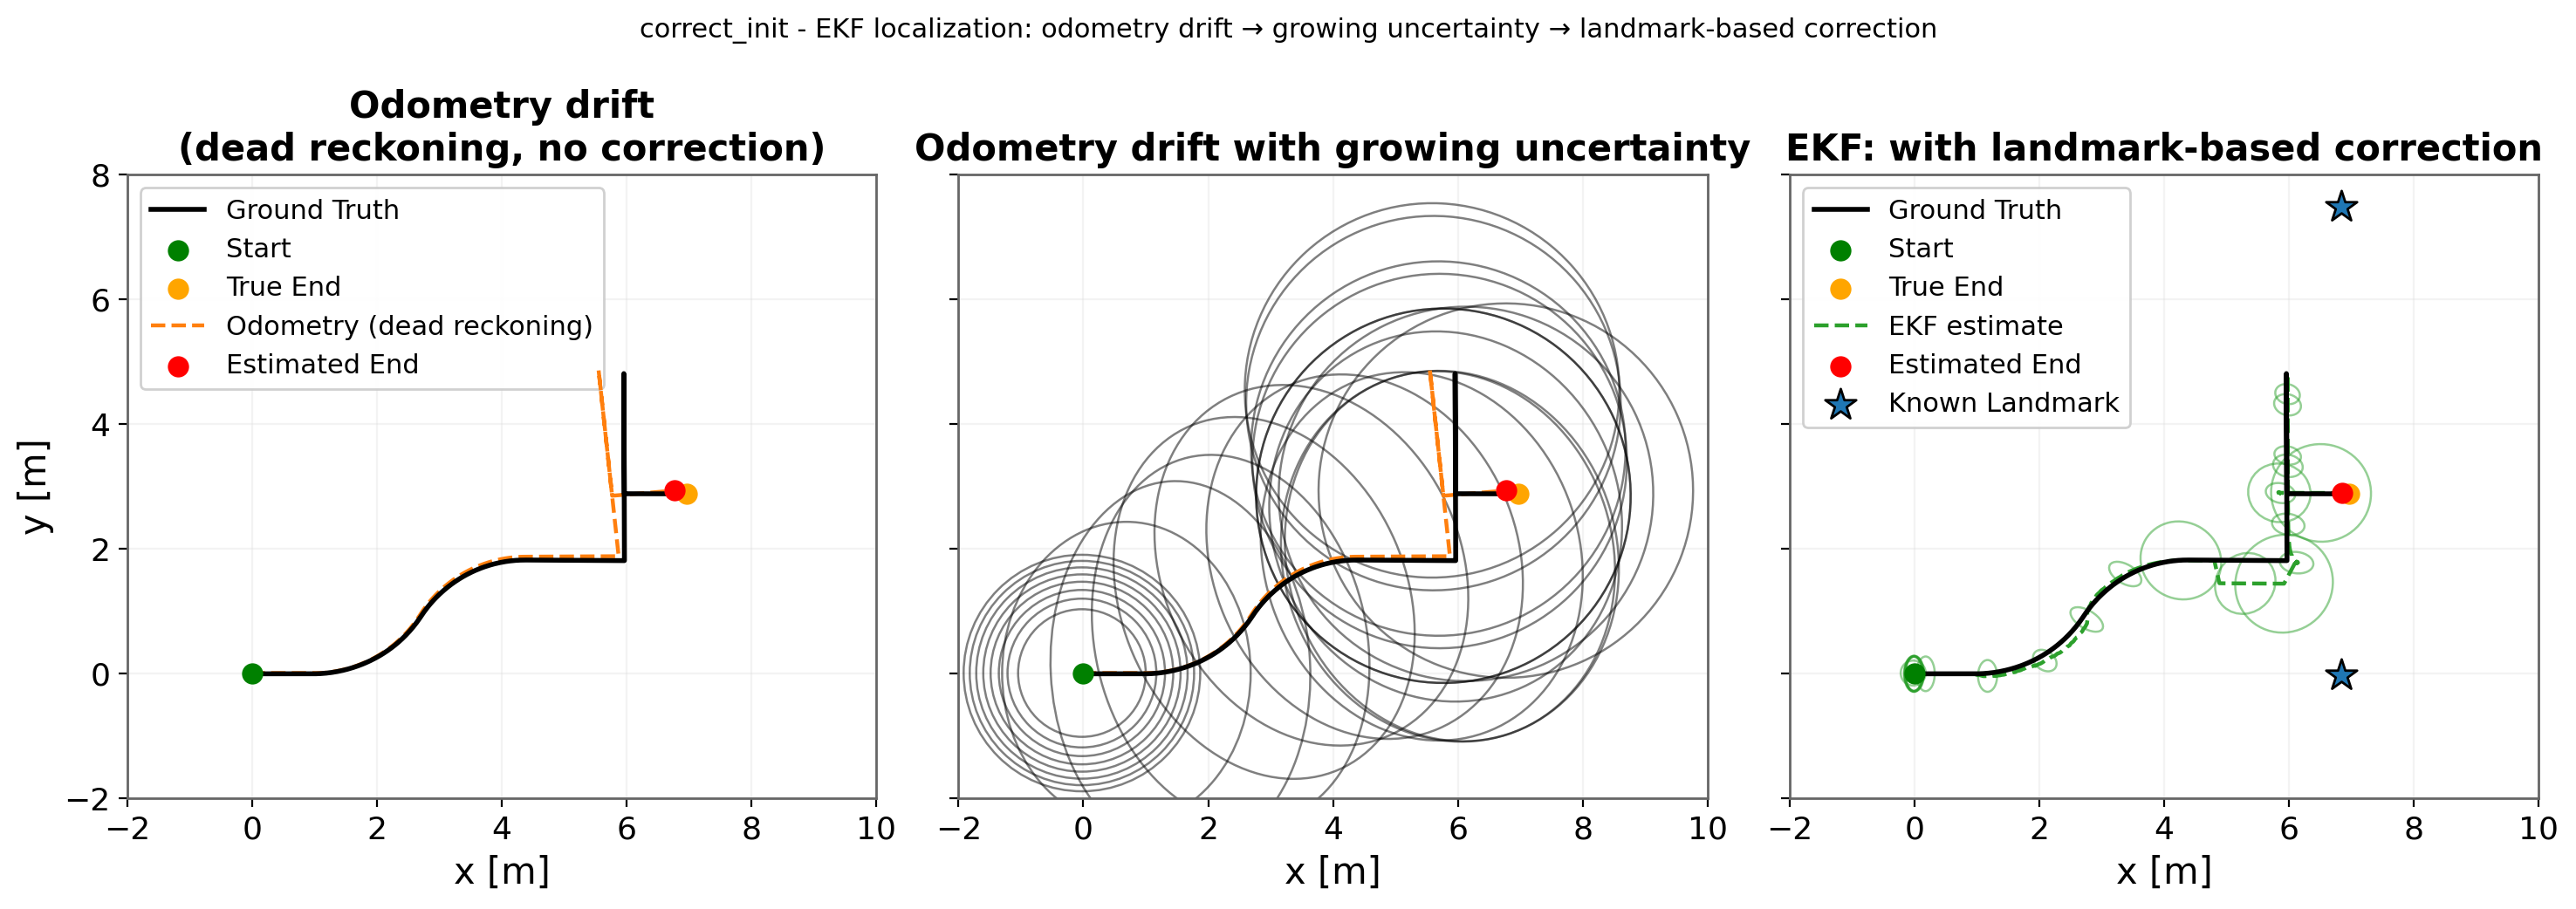
\includegraphics[width=0.92\textwidth]{images/correct_init_ekf_explainer.png}
    \caption{The localization principle, EKF, nominal scenario. Dead reckoning (left) drifts; its uncertainty grows without bound (centre, grey ellipses); landmark corrections (right, green) re-anchor the belief, keeping the estimated end pose (red) on the true end (orange). Stars mark the mapped AprilTag landmarks.}
    \label{fig:explainer}
\end{figure*}

\begin{table*}[!t]
\centering
\setlength{\tabcolsep}{0.5em}
{\renewcommand{\arraystretch}{1.25}
\begin{tabular}{|l|c|c|c|c|c|}
\hline
\textbf{Scenario} & \textbf{KF (landmark)} & \textbf{EKF (landmark)} & \textbf{EKF-LF (scan)} & \textbf{PF (scan)} & \textbf{AMCL (scan)} \\ \hline
\texttt{correct\_init}        & $0.11\pm0.01$ & $0.14\pm0.01$ & $0.15\pm0.01$ & $0.14\pm0.07$ & $0.15\pm0.17$ \\ \hline
\texttt{offset\_1m}           & $0.14\pm0.04$ & $0.15\pm0.01$ & $0.59\pm0.30$ & $0.31\pm0.05$ & $0.47\pm0.04$ \\ \hline
\texttt{offset\_5m}           & $\mathbf{0.30\pm0.27}$ & $0.30\pm0.22$ & $5.54\pm1.58$ & $3.58\pm1.08$ & $4.13\pm1.02$ \\ \hline
\texttt{wrong\_yaw\_pi2}      & $0.18\pm0.15$ & $\mathbf{0.14\pm0.01}$ & $0.16\pm0.02$ & $0.35\pm0.07$ & $0.45\pm0.02$ \\ \hline
\texttt{overconfident\_wrong} & $\mathbf{0.29\pm0.14}$ & $0.38\pm0.16$ & $5.05\pm1.11$ & $3.40\pm0.16$ & $2.98\pm0.23$ \\ \hline
\texttt{underconfident}       & $0.32\pm0.28$ & $\mathbf{0.27\pm0.19}$ & $4.17\pm3.09$ & $1.69\pm2.30$ & $0.51\pm0.03$ \\ \hline
\texttt{kidnapped}            & $\mathbf{2.62\pm1.00}$ & $2.99\pm1.12$ & $17.47\pm6.95$ & $9.21\pm3.89$ & $15.18\pm1.47$ \\ \hline
\end{tabular}}
\caption{Final position error RMSE$_{xy}$ in metres (mean $\pm$ one standard deviation over ten seeds). Landmark-identity filters (KF, EKF) recover from every adverse start; scan-based filters (EKF-LF, PF, AMCL) diverge once initialization is grossly wrong or the robot is kidnapped. Best per row in bold.}
\label{tab:rmse}
\end{table*}

\subsection{The localization principle}
Fig.~\ref{fig:explainer} contrasts the three regimes for the EKF in the nominal case. Pure dead reckoning drifts and, decisively, its uncertainty grows without bound: the filter does not know that it is wrong. Landmark observations periodically collapse the covariance and re-anchor the belief on the true trajectory. This bounded-uncertainty property, not raw accuracy, is what landmarks buy, as the results below make explicit.

\subsection{Recovery from adverse initialization}
Table~\ref{tab:rmse} and Fig.~\ref{fig:rmse} are the core result. Under nominal initialization all five filters localize to within $0.11$--$0.15$\,m and track the true path tightly across all seeds (Fig.~\ref{fig:traj_nominal}): when the start is correct, the sensing modality is irrelevant. The picture inverts sharply as the initial error grows. For a $5$\,m offset the landmark filters stay at $0.30$\,m while the scan filters degrade to $3.6$--$5.5$\,m, drifting into a wrong but symmetric bay; with an overconfident wrong prior the gap is $0.3$\,m versus $3$--$5$\,m. The effect is starkest under kidnapping (Fig.~\ref{fig:kidnap}): the landmark EKF re-localizes to the new pose as soon as its camera reads a tag at the new location, ending at $2.6$--$3.0$\,m RMSE (dominated by the search interval, not the final error), whereas EKF-LF, PF, and AMCL diverge to $9$--$17$\,m. Notably, \texttt{offset\_1m} and \texttt{wrong\_yaw\_pi2} are recovered by \emph{all} filters: a small or purely rotational error keeps the scan within the basin of attraction of the correct hypothesis, so aliasing does not yet dominate.

\begin{figure*}[!t]
    \centering
    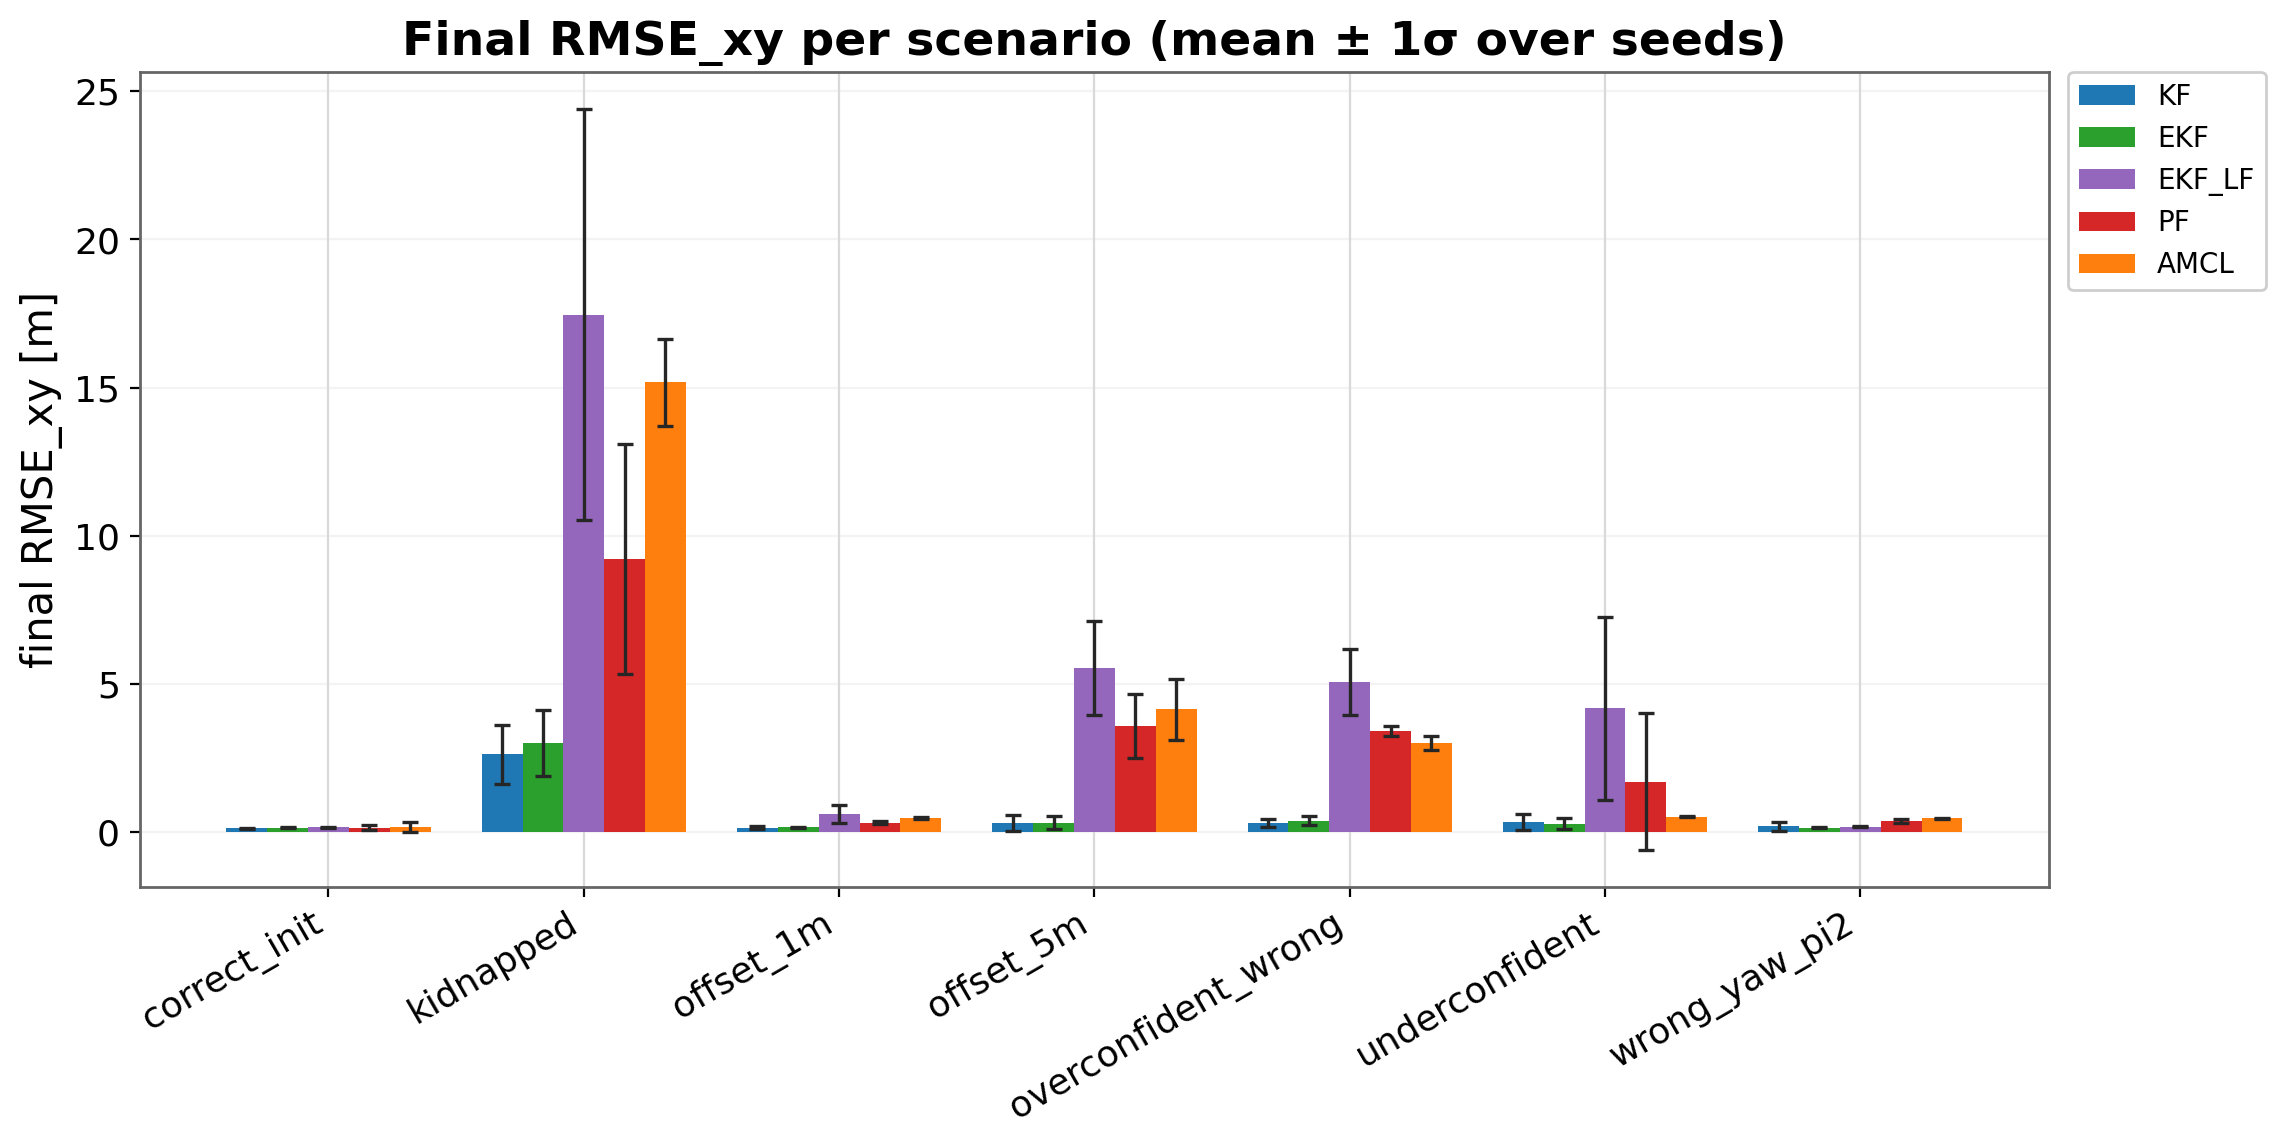
\includegraphics[width=0.92\textwidth]{images/rmse_comparison.png}
    \caption{Final RMSE$_{xy}$ per scenario (mean $\pm 1\sigma$, ten seeds). The landmark filters (KF, EKF) remain low across every adverse scenario; the scan filters explode under \texttt{offset\_5m}, \texttt{overconfident\_wrong}, and \texttt{kidnapped}.}
    \label{fig:rmse}
\end{figure*}

\begin{figure}[!t]
    \centering
    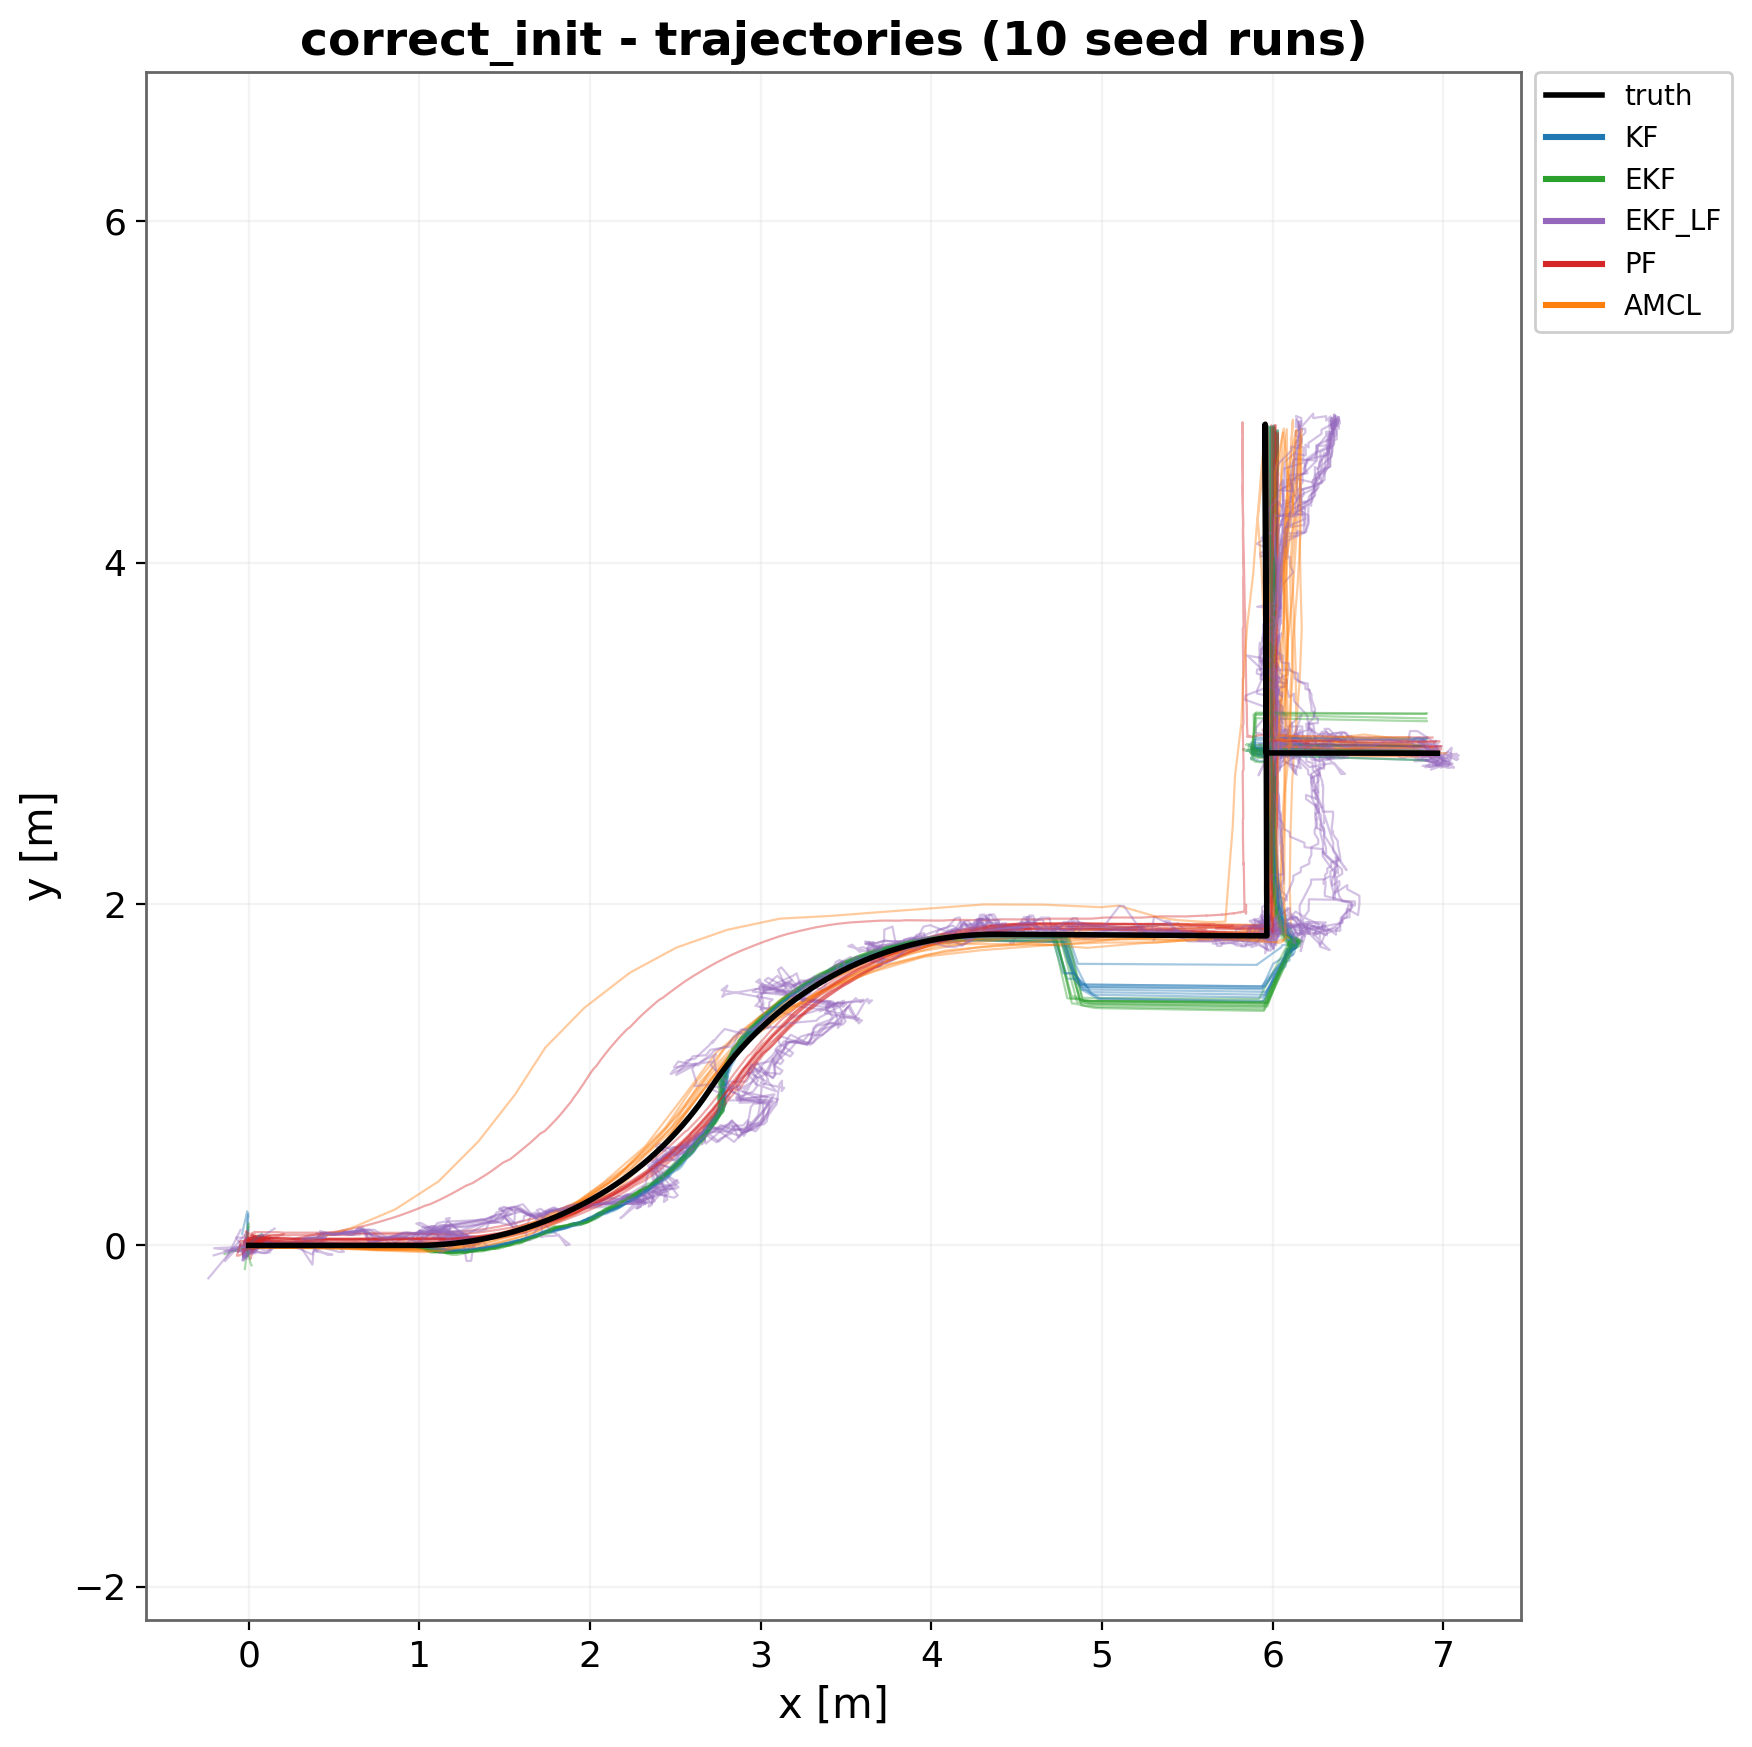
\includegraphics[width=\columnwidth]{images/correct_init_trajectory.png}
    \caption{Baseline (\texttt{correct\_init}), all ten seeds overlaid. With a correct start every filter tracks the true path tightly regardless of sensing modality --- the spread across seeds is small.}
    \label{fig:traj_nominal}
\end{figure}

\begin{figure*}[!t]
    \centering
    \begin{subfigure}{0.49\textwidth}
        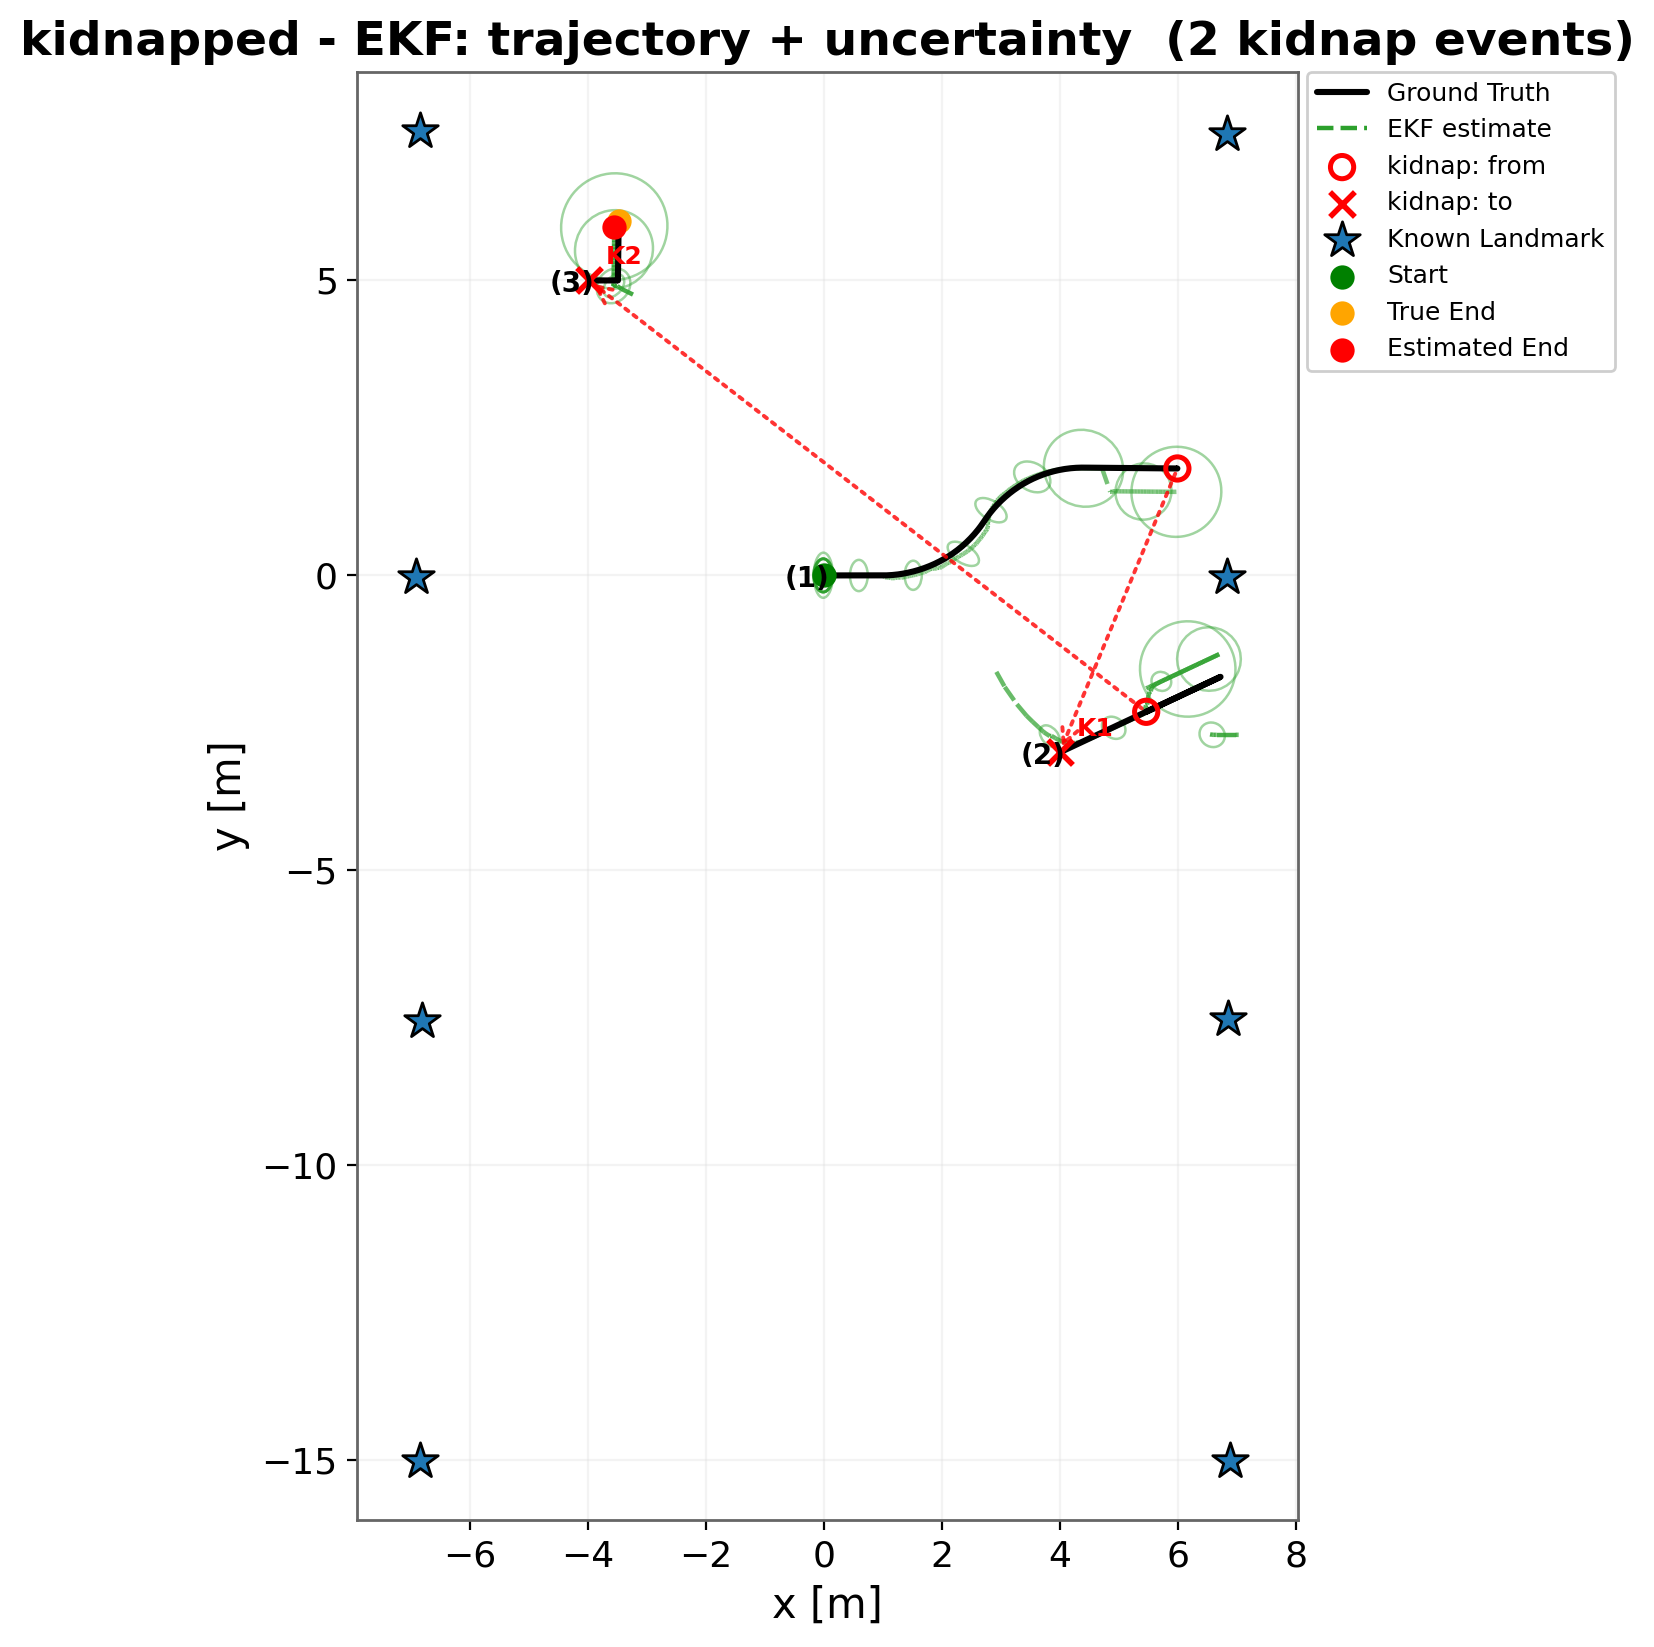
\includegraphics[width=\linewidth]{images/kidnapped_ekf_localization.png}
        \caption{EKF (landmark): recovers.}
    \end{subfigure}\hfill
    \begin{subfigure}{0.49\textwidth}
        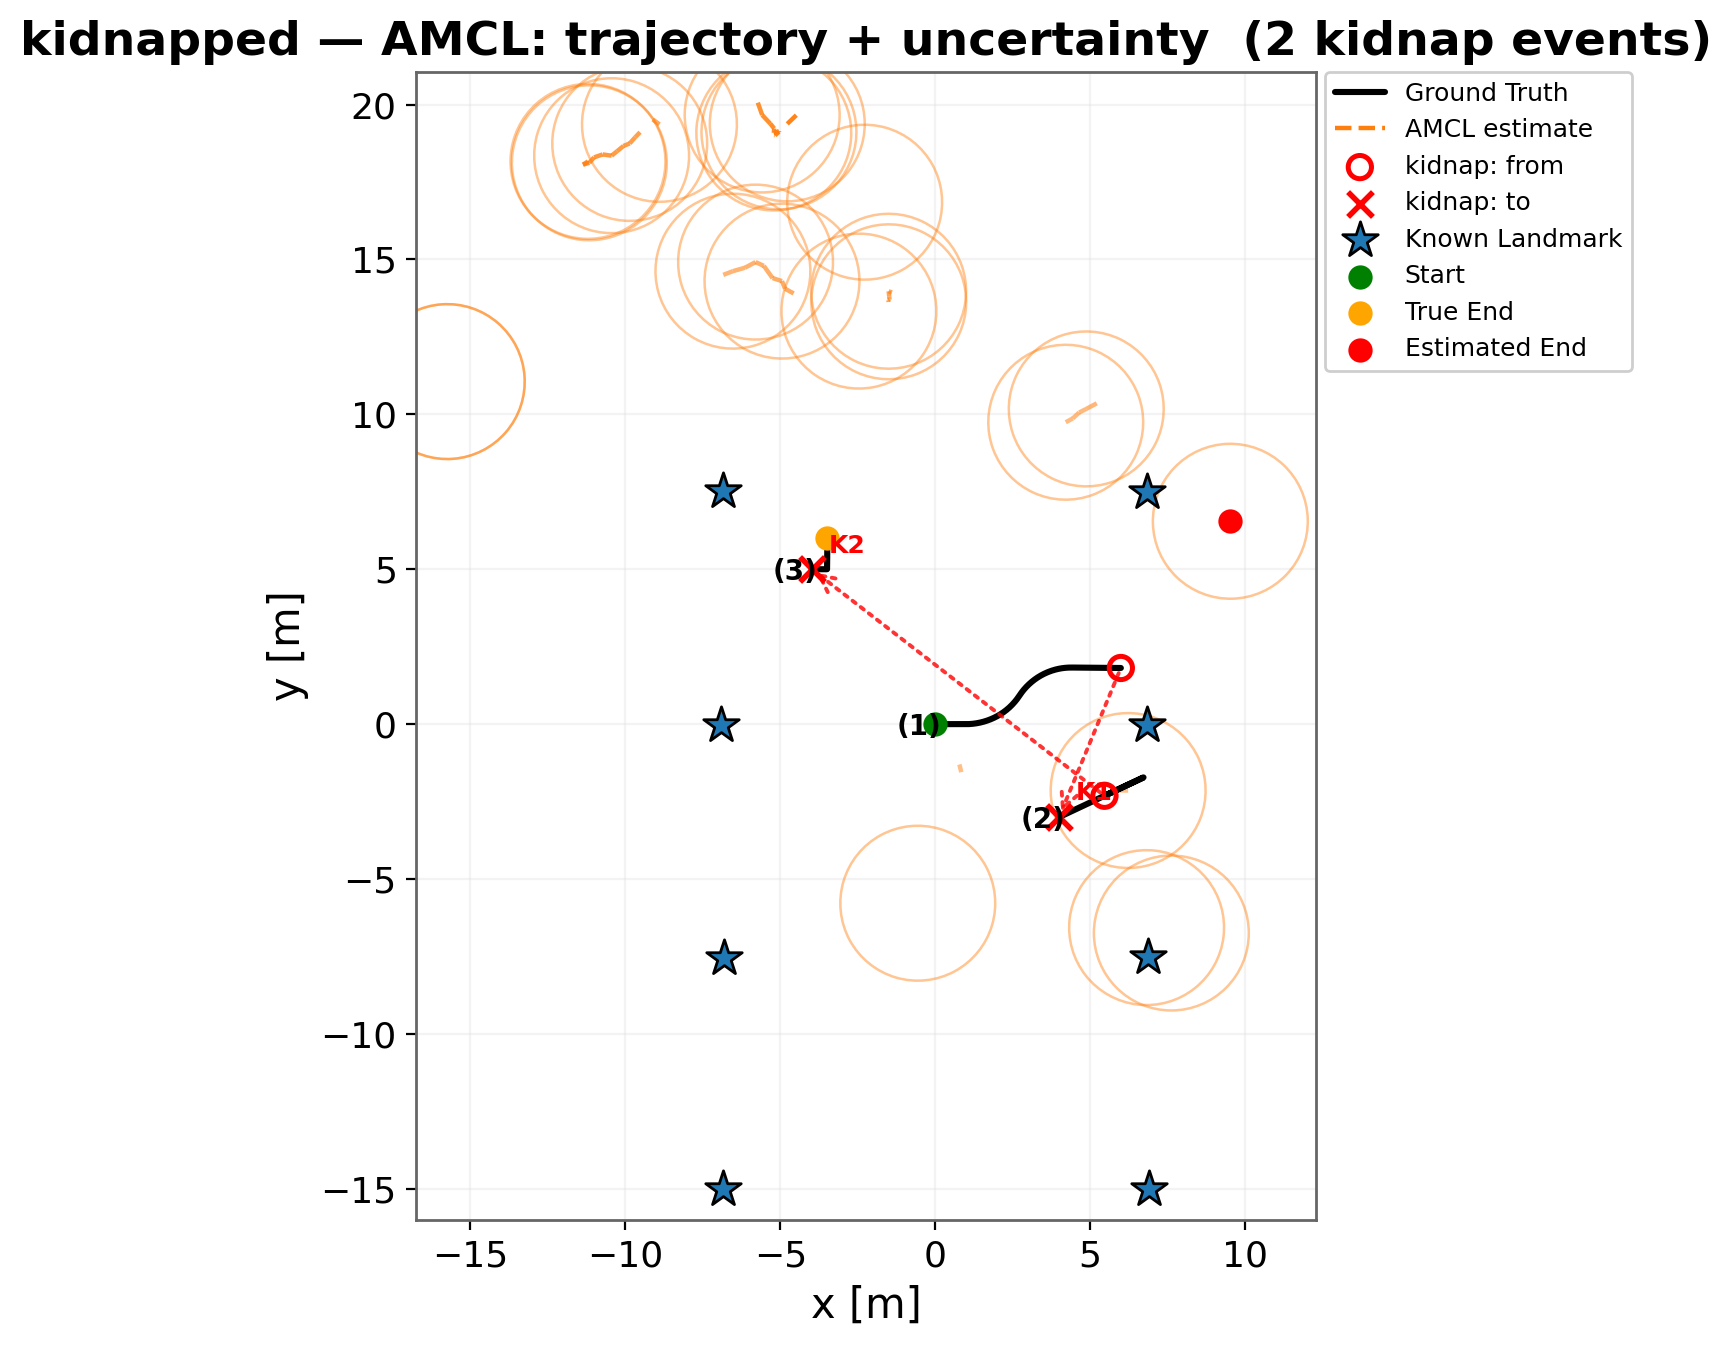
\includegraphics[width=\linewidth]{images/kidnapped_amcl_localization.png}
        \caption{AMCL (scan): diverges.}
    \end{subfigure}
    \caption{Kidnapped scenario, two teleports (markers K1, K2). The landmark EKF (left) snaps its estimated end pose (red) onto the true end (orange) once it reads a tag at the new location; the scan-based AMCL baseline (right) cannot disambiguate the symmetric map and is lost.}
    \label{fig:kidnap}
\end{figure*}

\subsection{Why scan filters fail: perceptual aliasing}
The scan filters are not poorly implemented; they are defeated by the environment. In the symmetric pillar grid, a forward displacement of one $7.5$\,m bay produces a near-identical scan, so the likelihood field admits several mutually distant maxima. A unimodal scan-EKF locks onto whichever maximum is nearest its (wrong) prior, and the particle filter, even with random injection, converges to a wrong but symmetric hypothesis. The convergence-rate plot (Fig.~\ref{fig:conv}) quantifies the stochasticity this induces: under kidnapping the landmark KF and EKF reach the $0.20$\,m criterion in $40\%$ and $60\%$ of seeds respectively, while no scan-based seed ever does. The landmark filters sidestep aliasing entirely because the tag identity in~(2) names the correct pillar a~priori; this is the honest, measurable analogue of the known-correspondence assumption~\cite{Neira2001}. The practical consequence is a human-in-the-loop asymmetry: the landmark filters recover autonomously, whereas the scan filters require an operator to supply a fresh initial belief, the familiar ``2D pose estimate'' of an interactive re-localization, before they reconverge. In other words, the particle filter still needs a reasonable initial guess to escape the aliased basin, exactly the global-localization limitation that augmented MCL only partially mitigates~\cite{Thrun2005}; identifiable landmarks remove this dependence on the operator. The textbook remedy fails here for two compounding reasons: under aliasing the symmetric twin keeps the scan likelihood high, so the kidnap is often \emph{not even detected} (the likelihood never drops, so no particles are injected), and when particles \emph{are} injected they simply reconverge to a symmetric-equivalent pose.

\begin{figure*}[!t]
    \centering
    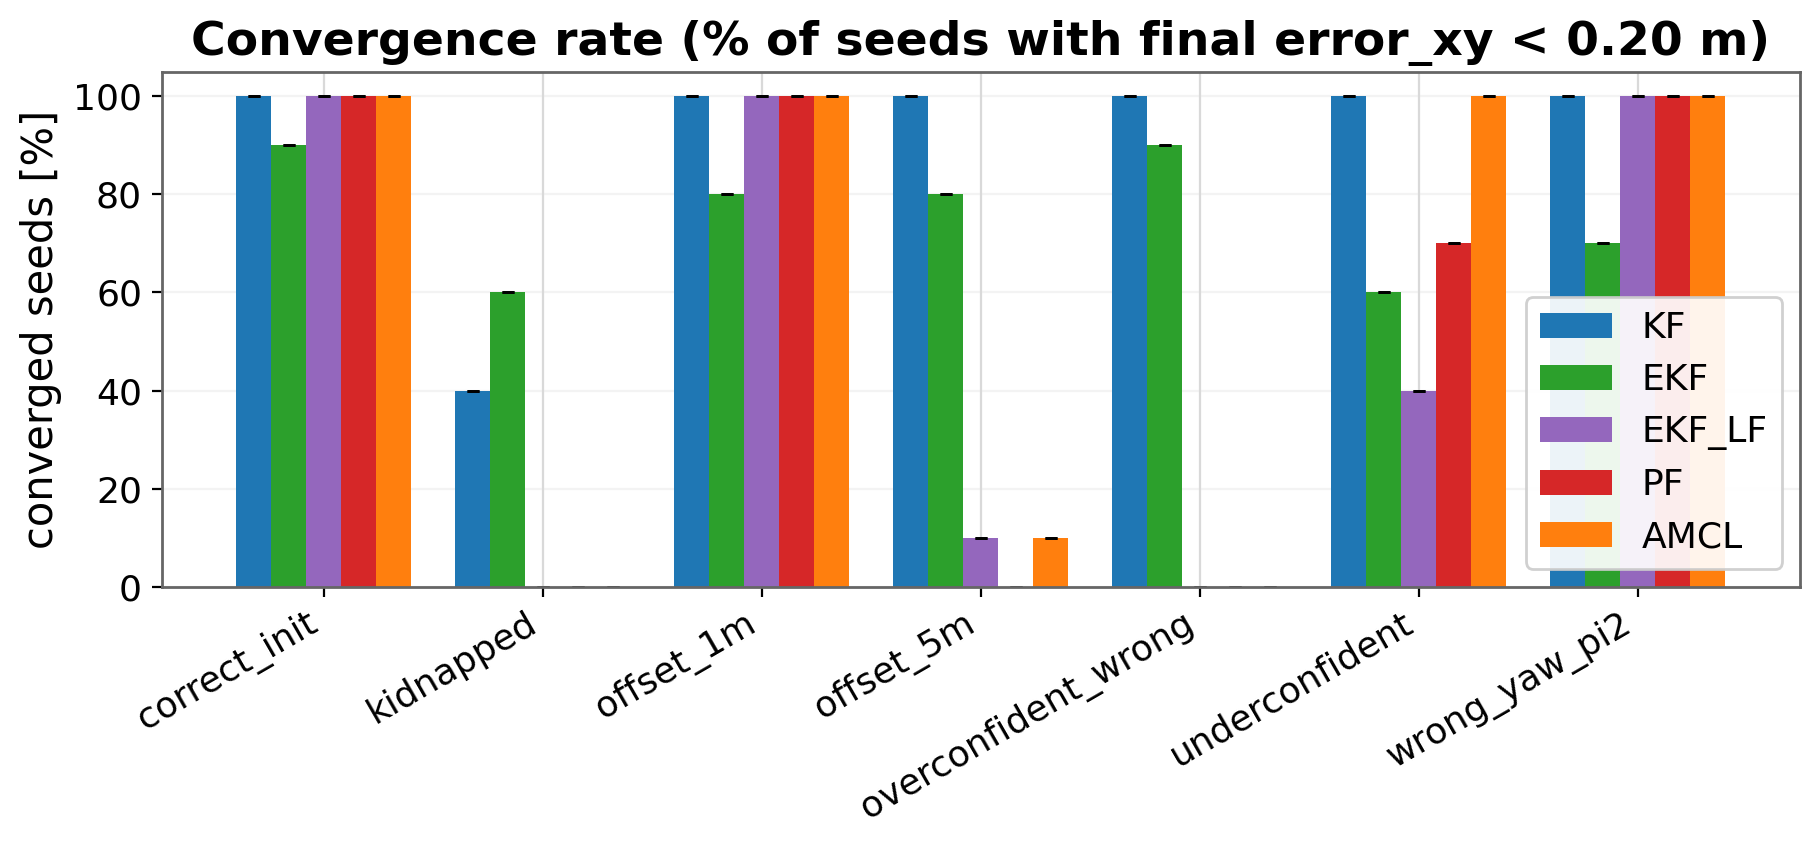
\includegraphics[width=0.92\textwidth]{images/convergence_rate.png}
    \caption{Convergence rate: percentage of seeds whose final position error is below $0.20$\,m. The landmark filters succeed in the adverse scenarios where the scan filters never converge; the partial kidnap recovery ($40$--$60\%$) reflects the stochastic search through the aliased map.}
    \label{fig:conv}
\end{figure*}

\subsection{The nominal-case caveat and cost}
The advantage of landmarks is specific to bad initialization. Under \texttt{correct\_init} the landmark EKF is no more accurate than dead reckoning would be over this short, low-drift trajectory; each measurement merely injects noise, and with a single visible tag the range--bearing update is a geometrically weak constraint. The benefit is robustness and bounded uncertainty, not nominal precision, an honest distinction we make explicit rather than hide. In terms of cost (Fig.~\ref{fig:runtime}), the Gaussian landmark filters are also the cheapest, at $\mathcal{O}(n^3)$ per update versus $\mathcal{O}(M\!\cdot\!R)$ for the sample-based filters over $M$ particles and $R$ rays; the landmark filters thus dominate on both robustness and computation in this setting.

\begin{figure*}[!t]
    \centering
    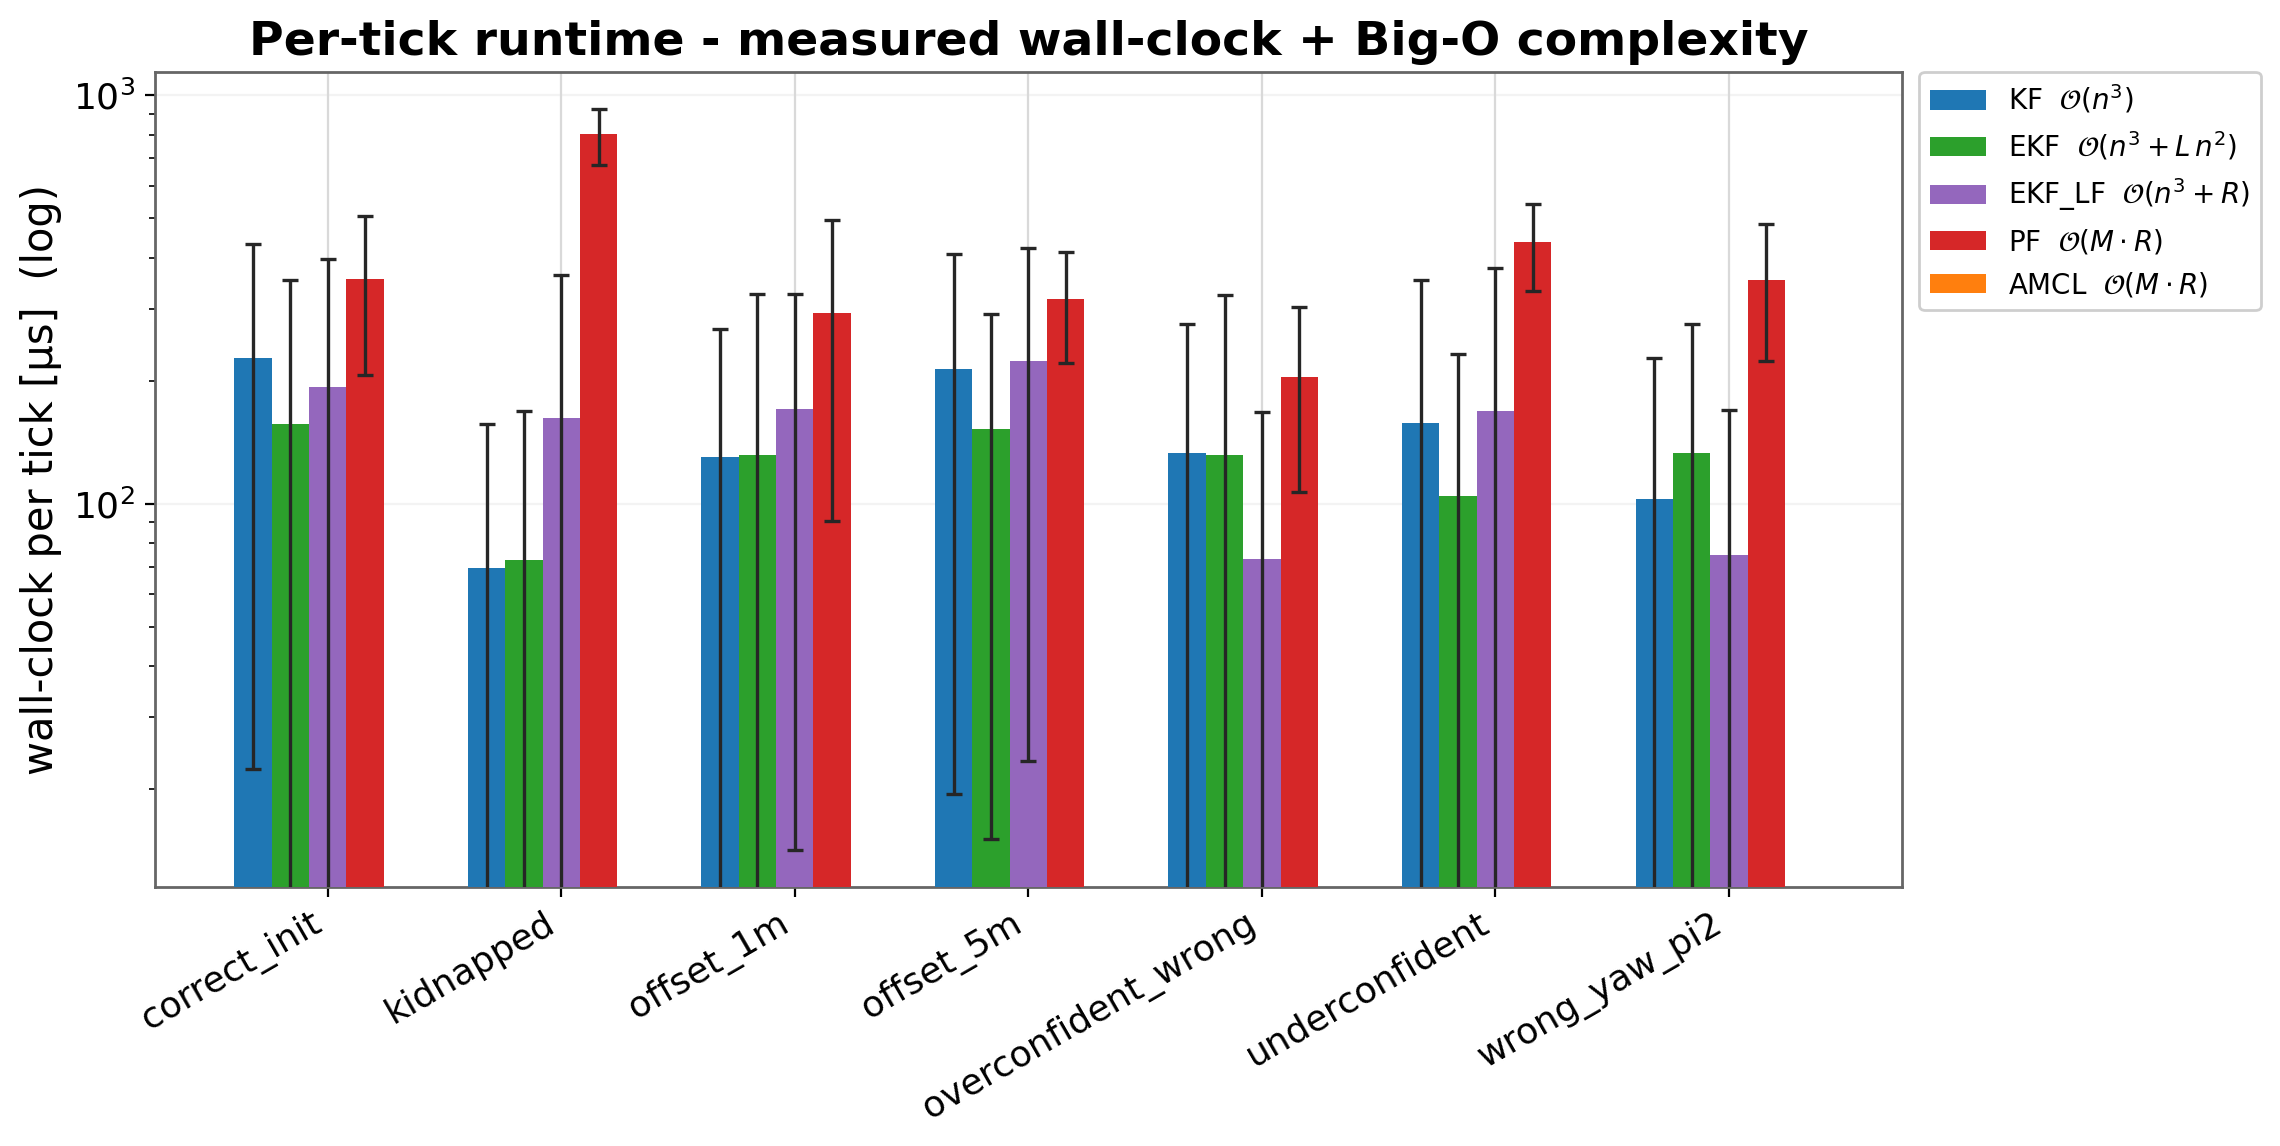
\includegraphics[width=0.92\textwidth]{images/runtime_comparison.png}
    \caption{Measured per-tick runtime (log scale) with asymptotic complexity. The Gaussian landmark filters are orders of magnitude cheaper than the sample-based scan filters.}
    \label{fig:runtime}
\end{figure*}

\subsection{Threats to validity}
The study is in simulation, so odometry is more benign than on hardware, which flatters dead reckoning in the nominal case. The forward-facing camera limits landmark visibility, a realistic but scenario-dependent constraint. Finally, fiducials require instrumenting the environment; our claim is not that tags are universally preferable but that, where identifiable landmarks are available, they convert the recovery problem from intractable to easy in exactly the aliased settings that defeat scan matching.

%%%%%%%%%%%%%%%%%%%%%%%%%%%%%%%%%%%%%%%%%%%%%%%%%%%%%%%%%%%%%%%%%%
\section{Summary and Outlook}

We compared five localization filters under seven adverse-initialization scenarios on a TurtleBot~4 in a perceptually symmetric warehouse, with the four research filters implemented from first principles and landmark identity measured honestly from camera-read AprilTags. Across ten seeds per scenario, filters that observe identifiable landmarks recovered from large offsets, wrong heading, miscalibrated covariance, and double kidnapping, whereas scan-based filters, including the Nav2 AMCL baseline, were defeated by perceptual aliasing and diverged by up to $17$\,m. The advantage was specific to bad initialization and disappeared under nominal conditions, where all filters localized to within $0.15$\,m. The decisive factor for recovery is therefore the identifiability of the observation model, not the sophistication of the estimator.

We deliberately kept the two modalities separate to isolate their effect; the natural next step is therefore to fuse them, using scans for nominal accuracy and tags for recovery, and to test on hardware, where odometry drift would further favour corrected filters. Making the scan filters self-recover in such symmetric maps needs richer global cues than the likelihood field: sensor-resetting or mixture proposals that draw hypotheses directly from the observation~\cite{Thrun2005}, appearance-based place recognition~\cite{Cummins2008,Lowry2016}, or multi-hypothesis tracking that follows all symmetric candidates until motion disambiguates. Active perception, in which the robot deliberately turns its limited-field-of-view camera toward an expected landmark after a likelihood collapse, is a further route to faster and more reliable kidnap recovery~\cite{Cadena2016}. The benchmark, simulation, and data are released to support reproducible follow-up work~\cite{Kummerle2009}.

%%%%%%%%%%%%%%%%%%%%%%%%%%%%%%%%%%%%%%%%%%%%%%%%%%%%%%%%%%%%%%%%%%
% Flush all pending figure floats before the references so the bibliography is
% always last (otherwise deferred full-width figures land after it).
\clearpage
{\small
\bibliographystyle{IEEEtranS}
\bibliography{refs}
}

\end{document}
